%\documentclass[10pt]{letter}
%\usepackage[utf8]{inputenc}

%%%%%%%%%%%%%%%%%%%%%%%%%%%%%%%%%%%%%%%%%%%%%%%%%
% compile with LuaLatex
%%%%%%%%%%%%%%%%%%%%%%%%%%%%%%%%%%%%%%%%%%%%%%%%%%%%%%%
\documentclass[11pt]{report}
\usepackage{epsfig}
\usepackage{amssymb,amsmath,amsfonts}
\usepackage[activeacute,american]{babel}
%\usepackage[utf8]{inputenc}
\usepackage{subfiles}
\usepackage{cite}
\usepackage{csquotes}
\usepackage{esvect}
\usepackage[acronym,nonumberlist]{glossaries}
\renewcommand{\acronymname}{Nomenclature}
\usepackage{multicol}
\usepackage{caption} 
\usepackage{float}
\usepackage[
    math-style=ISO,      % Upper Case Greek is in italics
    bold-style=ISO,      % Bold math is in italics
    partial=upright,     % nabla and partial upright
    nabla=upright,
  ]{unicode-math}
\topmargin 1.2cm 
\textwidth 16.1cm
\textheight 22.5cm
\oddsidemargin 0.7cm
\setcounter{tocdepth}{5}
\addtolength{\voffset}{-2.4cm}
\addtolength{\hoffset}{-0.5cm}

\usepackage{setspace}
%\doublespacing
\onehalfspacing
\usepackage{caption}
 \captionsetup[figure]{labelfont={bf},name={Figura},labelsep=period}
\usepackage{booktabs}

%%%%%%%%%%%%%%%%%%%%%%%%%%%%%%% 

%%%%%%%%%%%%%%%%%%%%%%%%%%%%%%% 
% citas
% \footnotetext{Mott, Robert L. Mecanica de Fluidos 6/e. Pearson educación, 2006.}
% \footnotetext{Pritchard, Philip J. Fox and McDonald’s Introduction to Fluid Mechanics (8th ed.). John Wiley $\&$ Sons. (2011).}
% \footnotetext{Munson, Bruce R., et al. "Fundamentals of Fluid Mechanics, John Wiley $\&$ Sons." Inc., USA (2006).}
\footnotetext{Çengel, Yunus A and Cimbala, John M "Fluid Mechanics Fundamentals and Applications, Mc Graw Hill Higher Education" (2006)}

%%%%%%%%%%%%%%%%%%%%%%%%%%%%%%% 
\captionsetup{labelformat=empty,labelsep=none}
%%%%%%%%%%%%%%%%%%%%%%%%%%%%%%%%%
\begin{document}
\begin{center}
\begin{Large}
\textbf{Coeficiente de arrastre cuerpos 2D}

\textit{$Re>10^4$, $C_D$ basado en el \'area frontal}

\vspace{-0.5cm}

\end{Large}



\begin{table}[!htb]
   
    \begin{minipage}[t]{.5\linewidth}
      \caption{}
      \centering
\begin{tabular}{ll}
\toprule
Forma & $C_D$ \\
\midrule
Vara cuadrada &  \\
\raisebox{-.5\height}{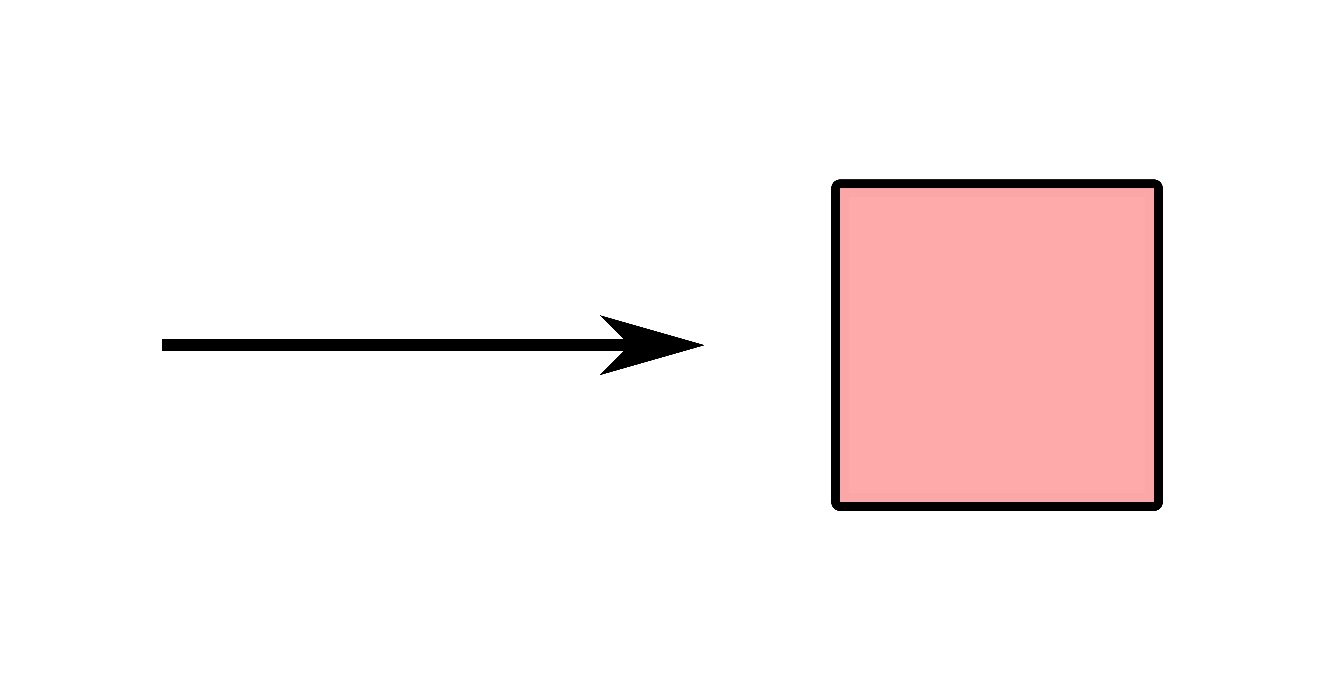
\includegraphics[width=4.5cm]{cuad1.eps}} & $2.1$\\
\raisebox{-.5\height}{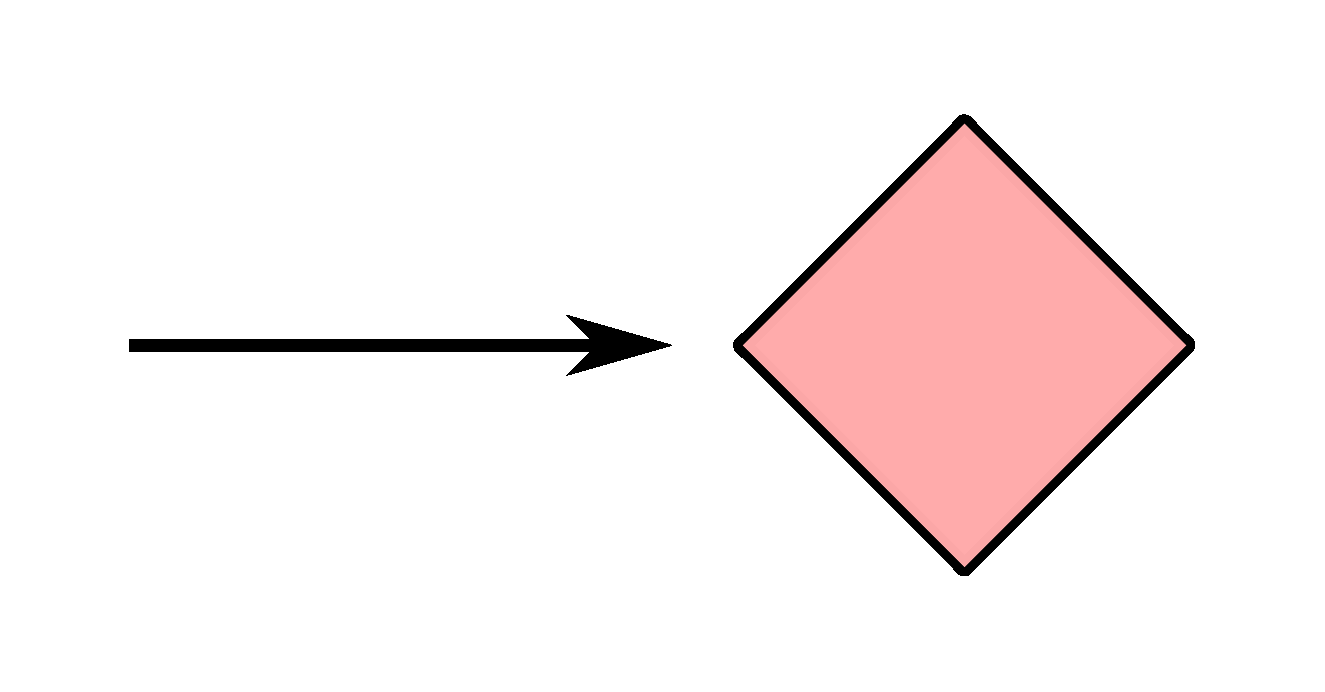
\includegraphics[width=4.5cm]{cuad2.eps}} & $1.6$\\
\midrule
Medio tubo & \\
\raisebox{-.5\height}{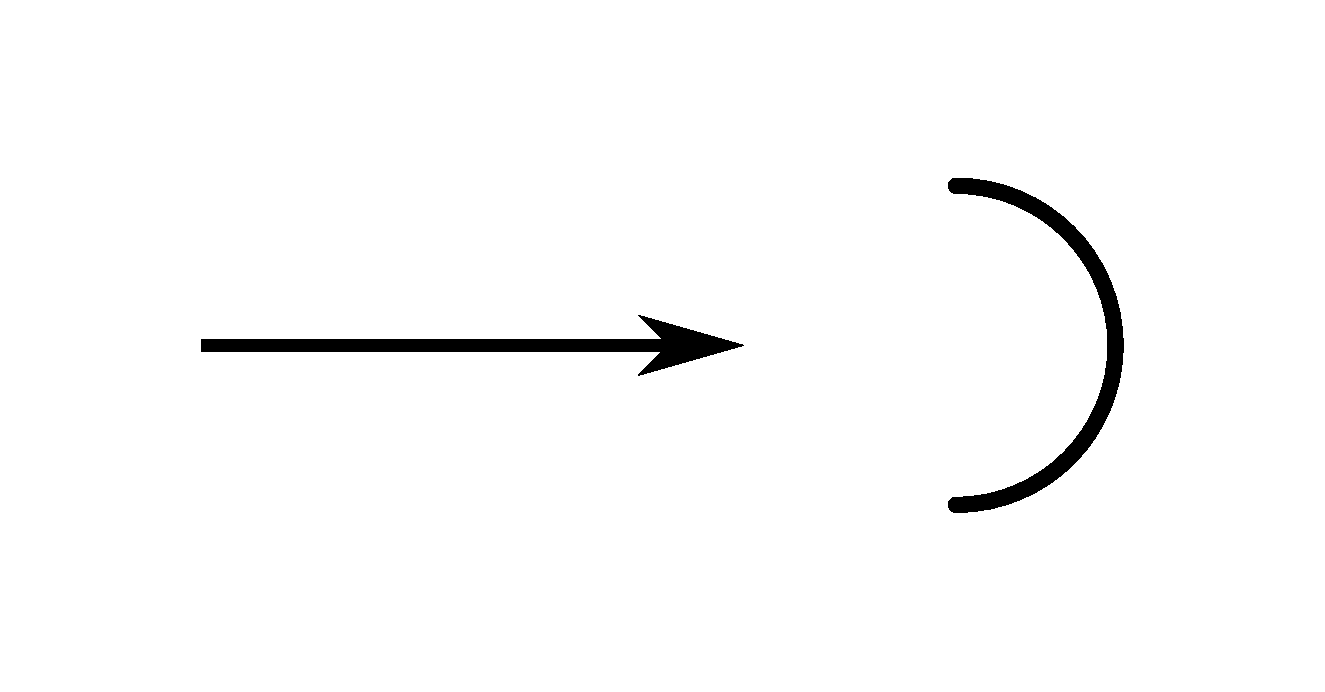
\includegraphics[width=4.5cm]{c1.eps}} & $1.2$\\
\raisebox{-.5\height}{\includegraphics[width=4.5cm]{c2.eps}} & $2.3$\\
\midrule
Medio cil\'indro & \\
\raisebox{-.5\height}{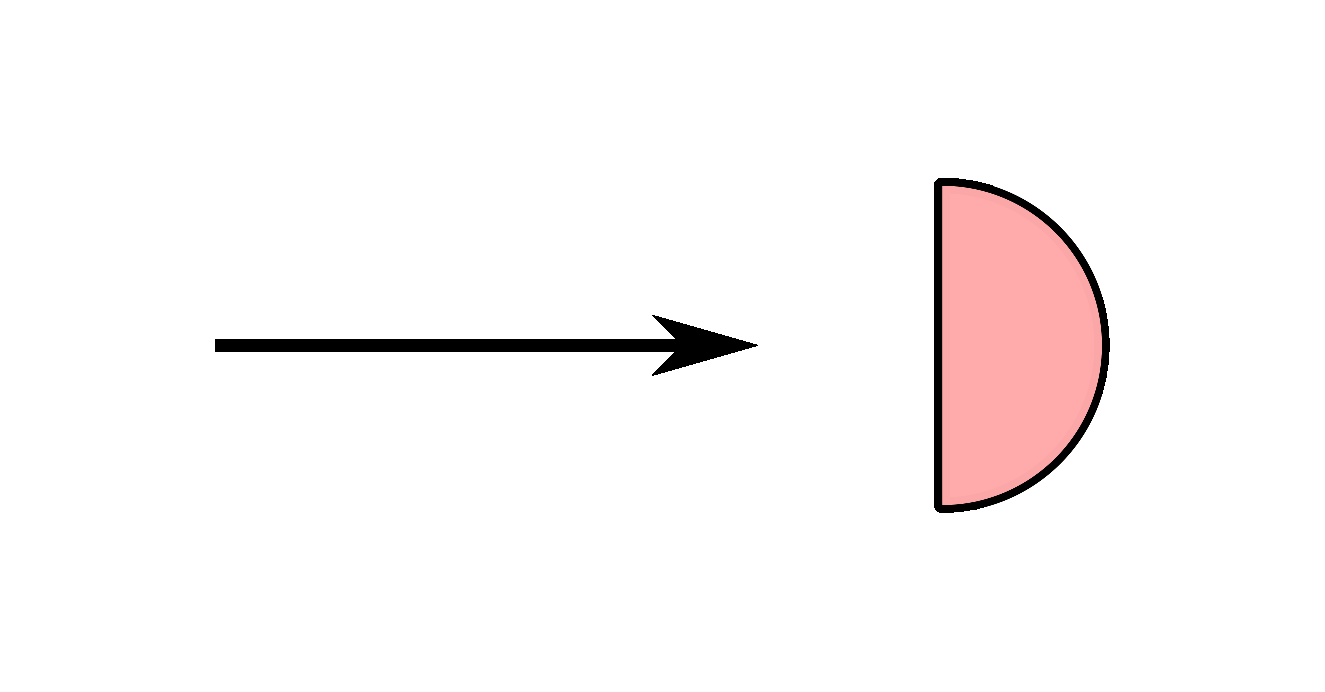
\includegraphics[width=4.5cm]{semi1.eps}} & $1.7$\\
\raisebox{-.5\height}{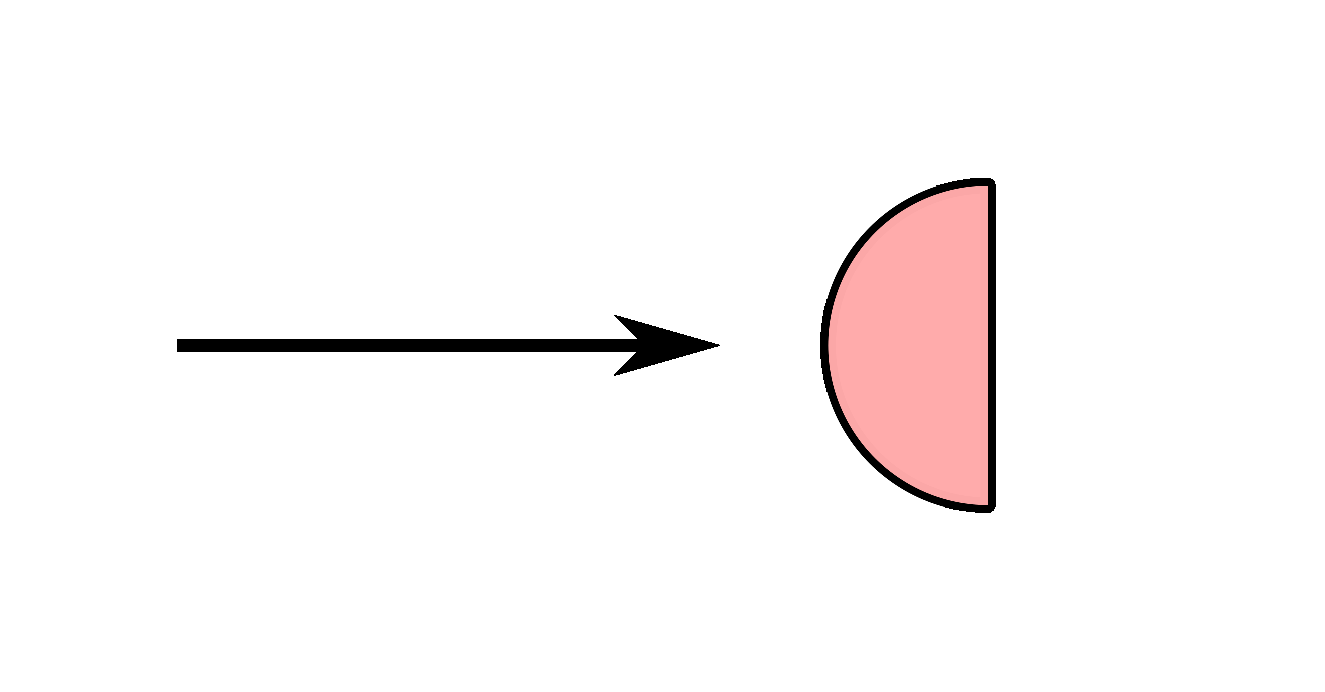
\includegraphics[width=4.5cm]{semi2.eps}} & $1.2$\\
\bottomrule
\end{tabular}
\end{minipage}%
\begin{minipage}[t]{.5\linewidth}
\centering
\caption{}
\begin{tabular}{ll}
\toprule
Forma & $C_D$ \\
\midrule
Tri\'angulo equil\'atero & \\
\raisebox{-.5\height}{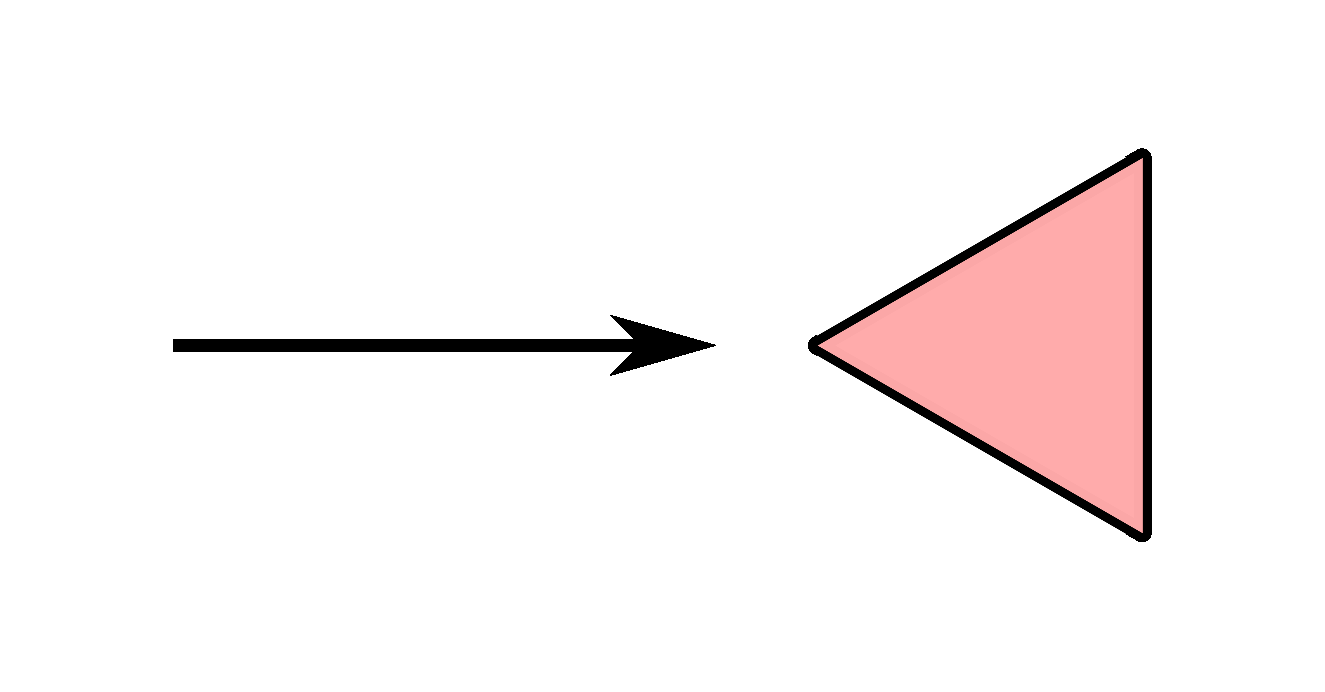
\includegraphics[width=4.5cm]{tri1.eps}} & $1.6$\\
\raisebox{-.5\height}{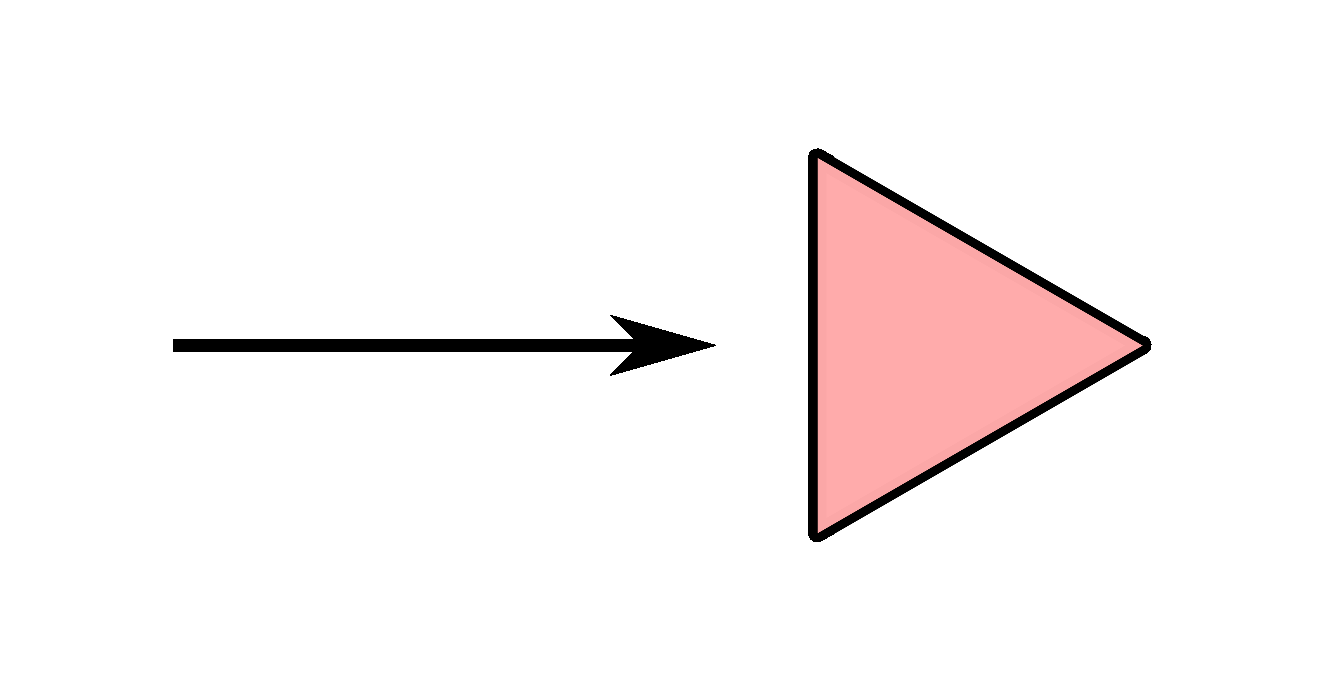
\includegraphics[width=4.5cm]{tri2.eps}} & $2.0$\\
\midrule
Hex\'agono & \\
\raisebox{-.5\height}{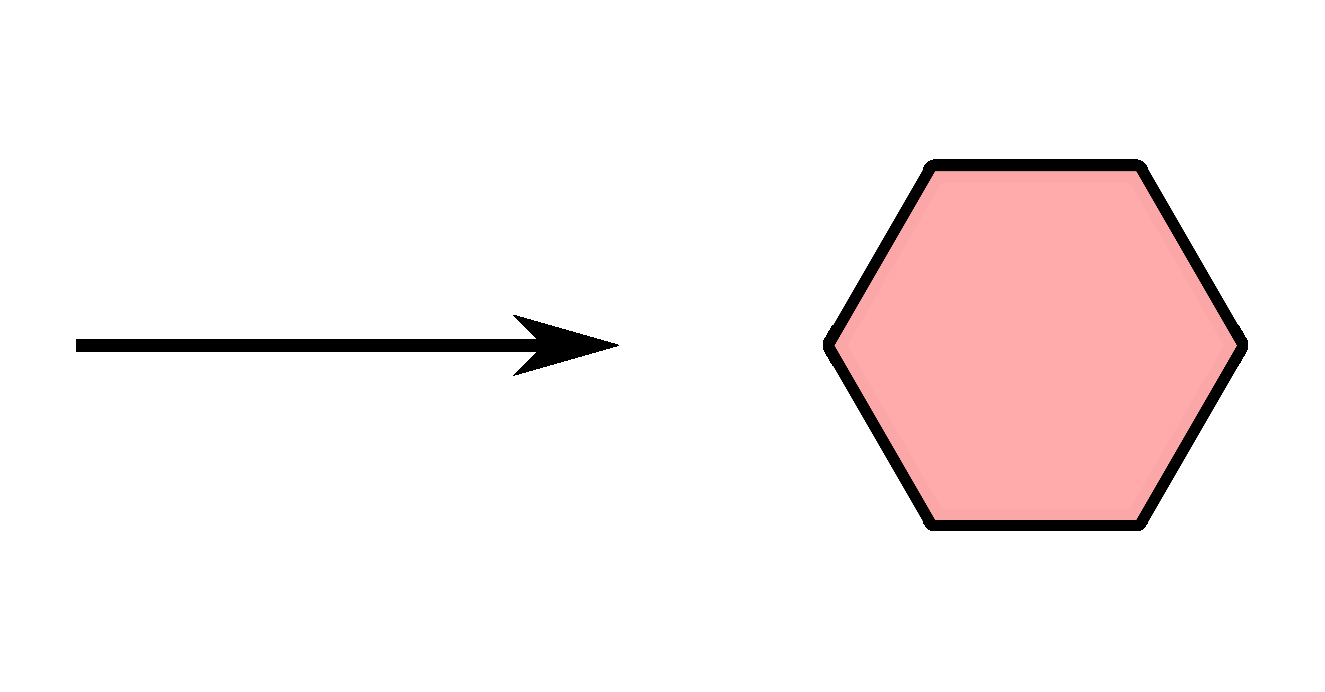
\includegraphics[width=4.5cm]{hex1.eps}} & $1.0$\\
\raisebox{-.5\height}{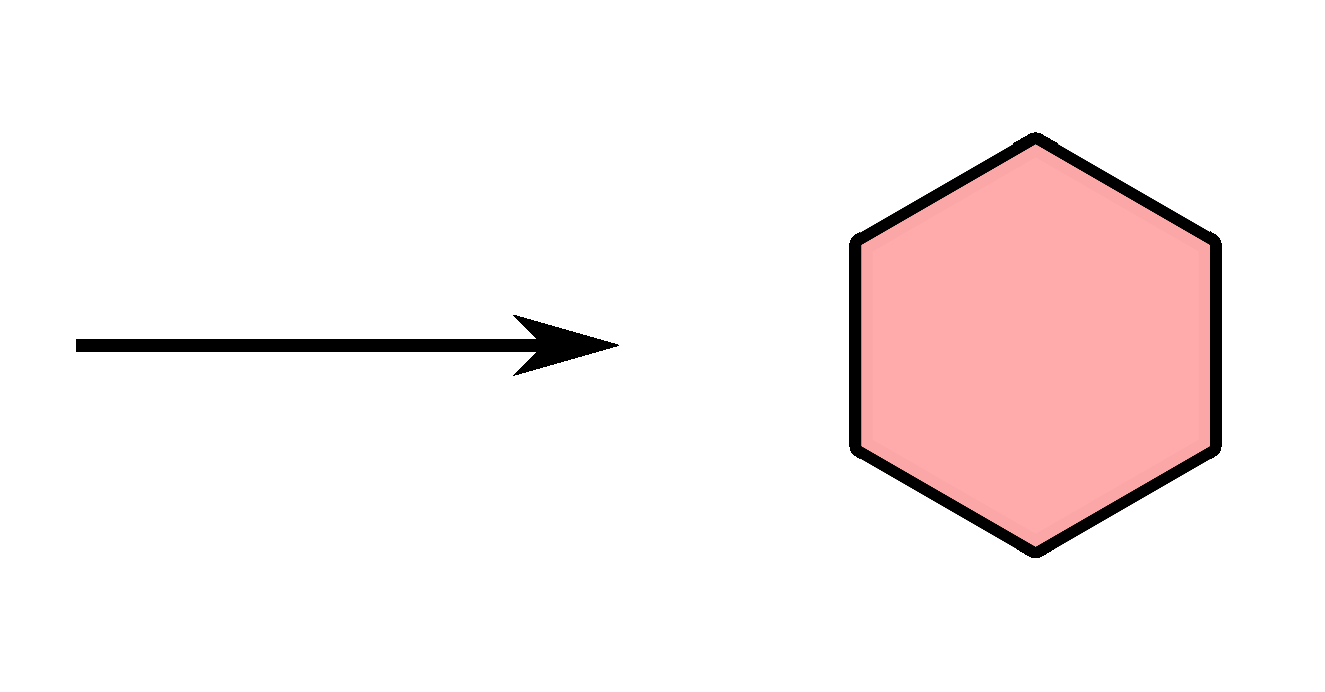
\includegraphics[width=4.5cm]{hex2.eps}} & $0.7$\\
\bottomrule 

\end{tabular}
\end{minipage} 
  
\end{table}

\end{center}
%%%%%%%%%%%%%%%%%%%%%%%%%

\newpage

%%%%%%%%%%%%%%%%%%%%%%%%%
%%%%%%%%%%%%%%%%%%%%%%%%%
%%%%%%%%%%%%%%%%%%%%%%%%%
\end{document}

